\subsection{Validazione e collaudo}
Il periodo di validazione e collaudo ha inizio il giorno 01-05-2021, in seguito alla conclusione dello sviluppo del prodotto, con termine fissato per il giorno 17-05-2021.
\subsubsection{Periodi e attività}
Questa fase si compone di un unico periodo, dal 01-05-2021 al 17-05-2021. Comprende attività di:
\begin{itemize}
	\item \textbf{Incremento e verifica dei documenti:} se fosse necessario, i documenti prodotti dal team verranno integrati;
	\item \textbf{Verifica e collaudo:} vengono creati e applicati un set di test, che hanno lo scopo di portare il prodotto ad un buon livello qualitativo. Il gruppo si focalizzerà sulla sua correttezza e nel rispetto di tutti i requisiti;
	\item \textbf{Codifica:} rilascio dell'ultima versione del prodotto.
\end{itemize}
\begin{figure}[h]
	\centering
	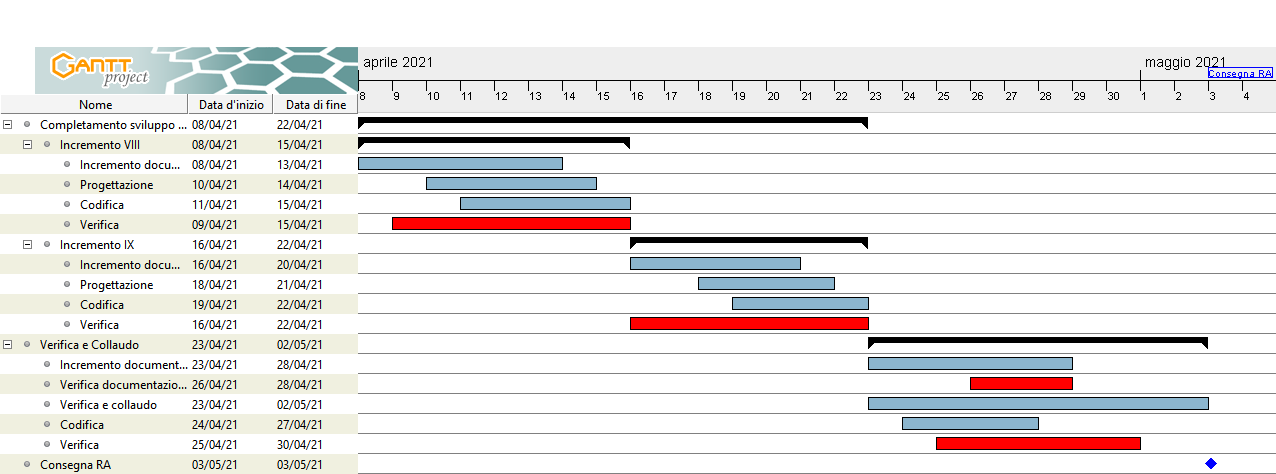
\includegraphics[width=\linewidth]{Images/GanttPianificazioneValidazioneCollaudo.PNG}
	\caption{Diagramma di Gantt dell'attività di validazione e collaudo}
\end{figure}


